\chapter{Another Use case}\label{ch:usecase}
To demonstrate that we achieved Research Goal \ref{item:goal:generic}, we implemented a different use case, called \textit{Plateforme DD}. The goal was to visualize the links between the content of the website\footnote{https://sciences.brussels/dd/} \textcolor{red}{TODO: meer uitleg geven over de bedoeling.}. The visualization and functionality is completely different from the one for GuideaMaps. The visualization for the map can be seen in Figure \ref{fig:plateforme-dd}.\\

\begin{figure}[H]
	\centering
	\frame{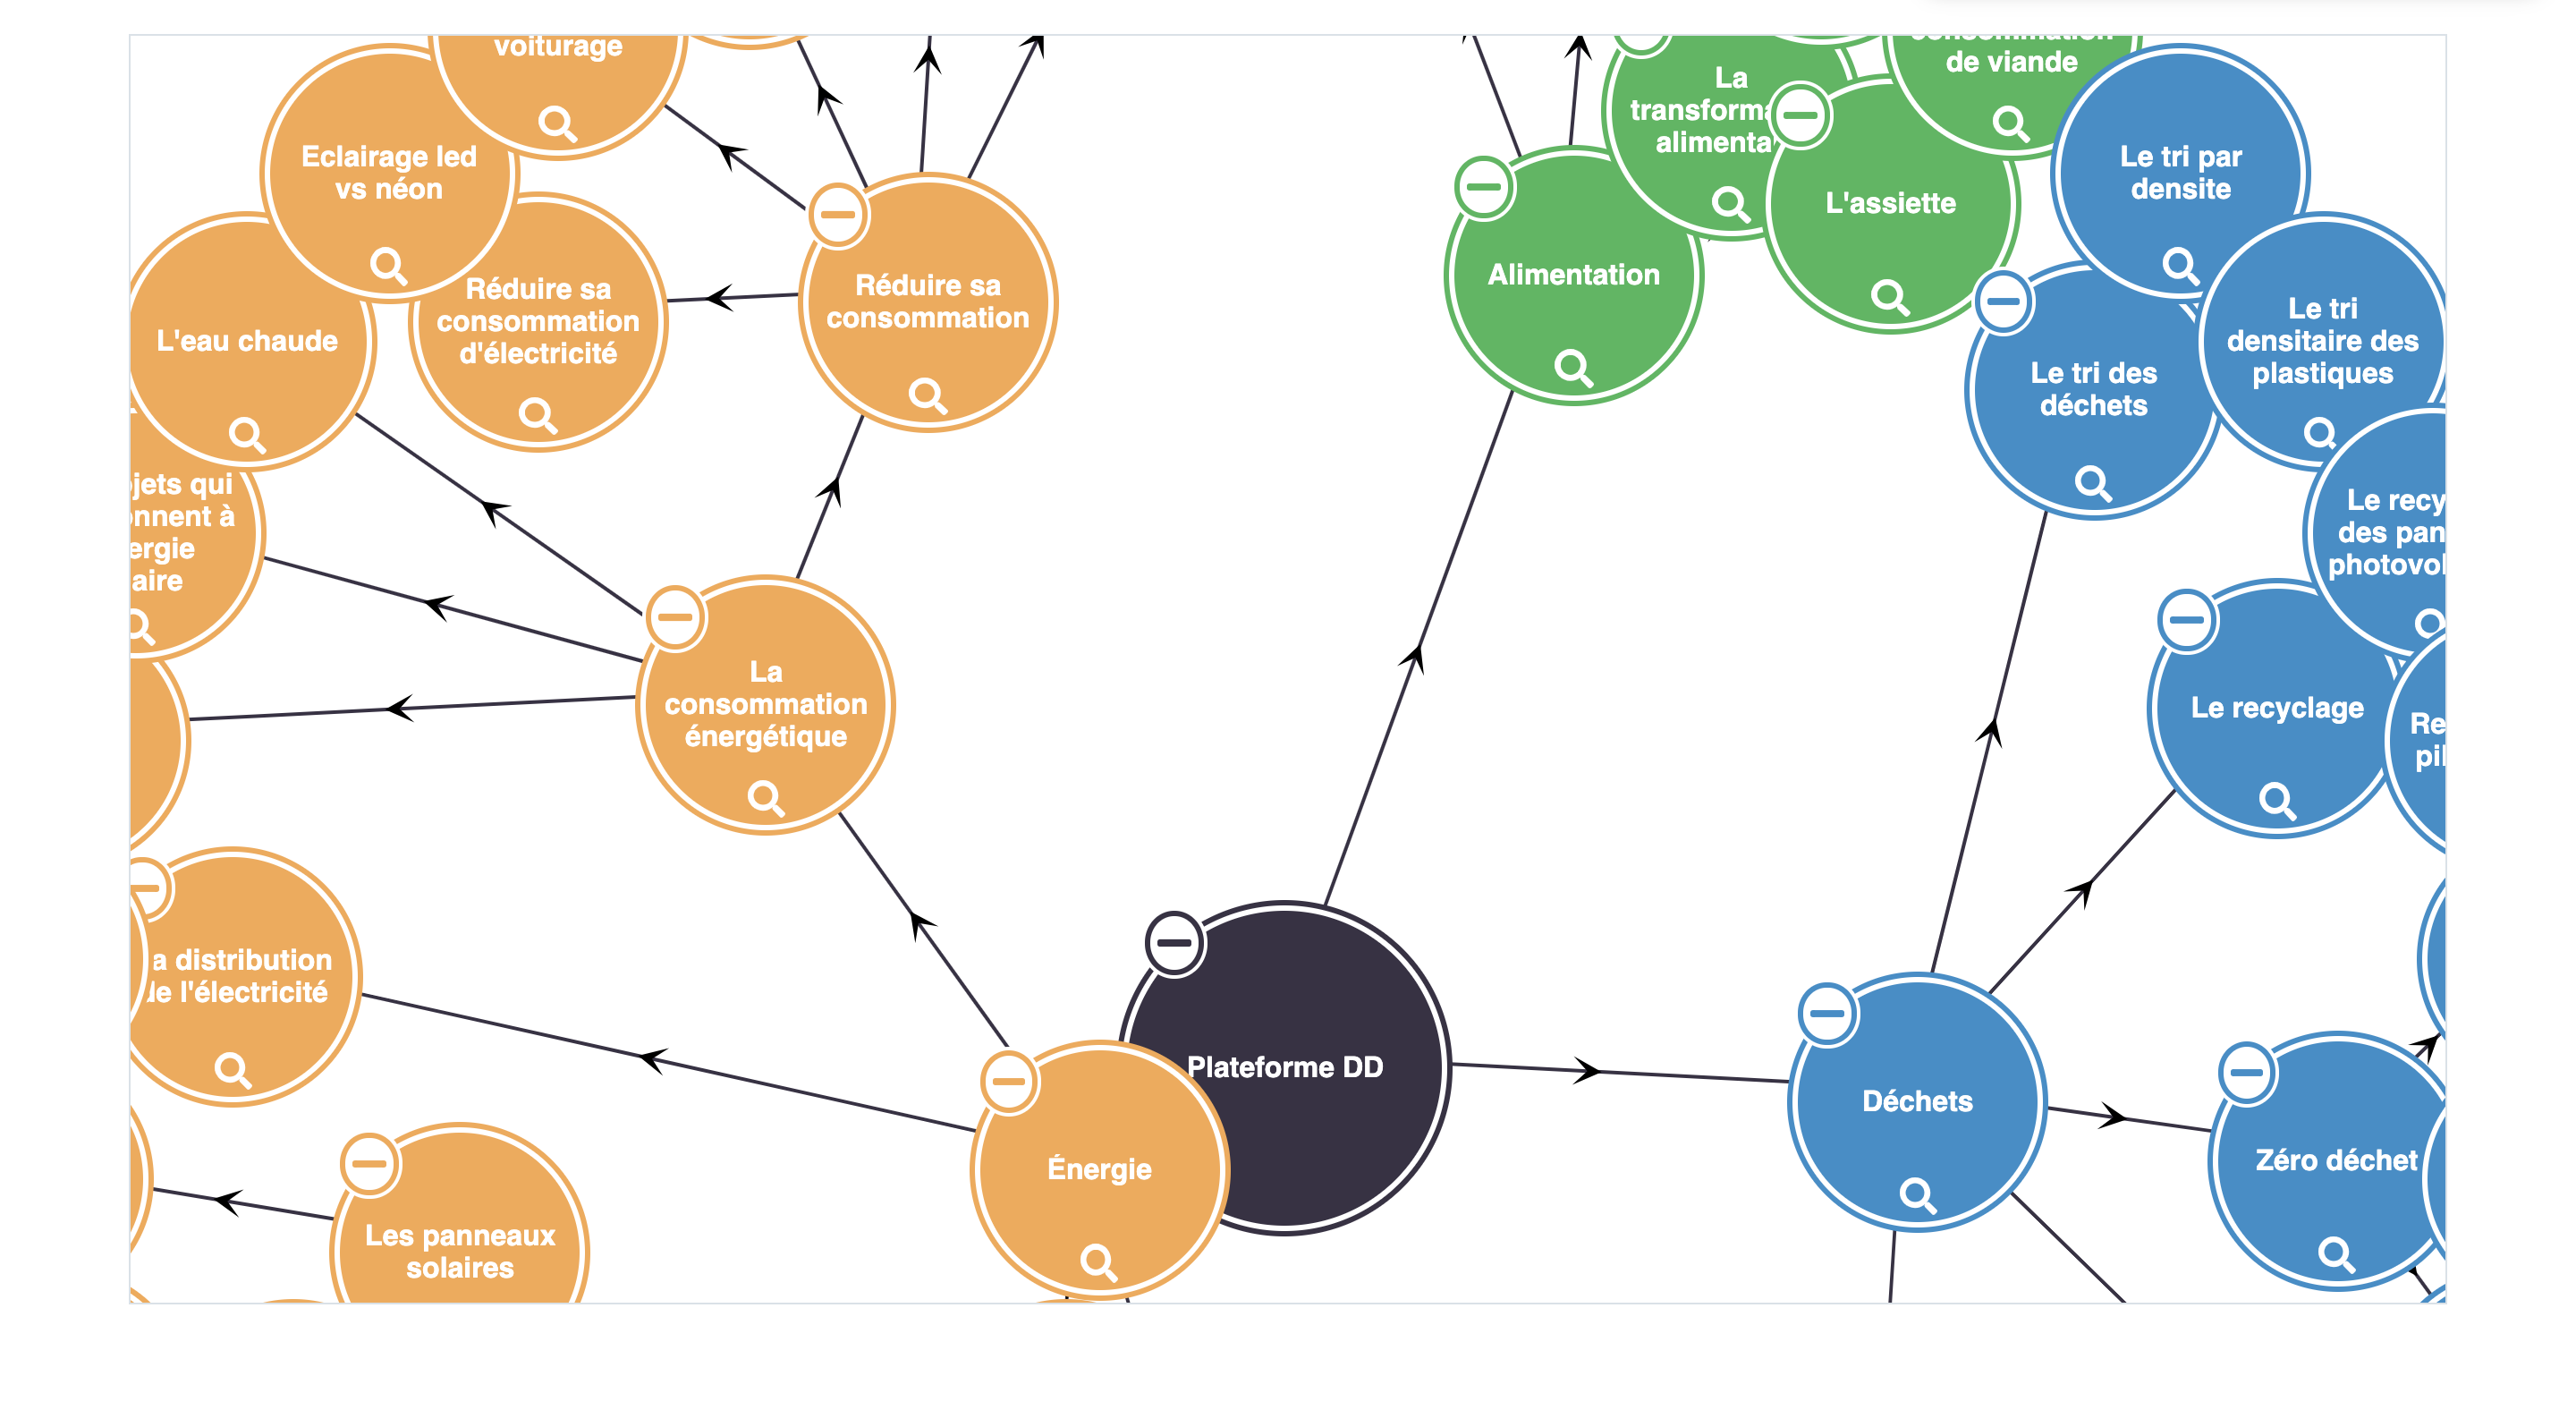
\includegraphics[width=\linewidth]{plateforme-dd.png}}
	\caption{Plateforme DD Layout.}
	\label{fig:plateforme-dd}
\end{figure}



\section{Configuration}\label{sec:usecase-configuration}
In Figure \ref{fig:examplecode-library}, we showed how we could alter the visualization of the data without affecting the default code. Remember that the props in that figure are not the only customizable props of the library. Figure \ref{fig:differences-gm-vs-pdd} shows the differences in configuration when we compare the visualization of GuideaMaps with the one of Plateforme DD.

\begin{figure}[H]
	\begin{minipage}{0.5\textwidth}
 		 \centering
		 \begin{minted}[breaklines, linenos, escapeinside=||]{html}
<ZoomableTree
    |\textcolor{mygreen}{NodeComp}|=|\textcolor{red}{\{GMNode\}}|
    |\textcolor{mygreen}{LinkComp}|=|\textcolor{red}{\{GMLink\}}|
    |\textcolor{mygreen}{EditModalComp}|=|\textcolor{red}{\{ GMEditModal\}}|
    |\textcolor{mygreen}{onAddNode}|=|\textcolor{red}{\{addGMNode\}}|
    |\textcolor{mygreen}{onDeleteNode}|=|\textcolor{red}{\{ deleteGMNode\}}|
    |\textcolor{mygreen}{onNodeUpdate}|=|\textcolor{red}{\{args -> updateGMNode(args)\}}|
    |\textcolor{mygreen}{onVisibleChildrenUpdate}|=|\textcolor{red}{\{ nodeId => updateGMVisibleChildren( nodeId)\}}|
/>
		\end{minted}
		\label{lst:default-components}
		\captionof{lstlisting}{GM Configuration.}
	\end{minipage}
 	\begin{minipage}{0.5\textwidth}
  		\centering
  		\begin{minted}[breaklines, escapeinside=||]{html}
<ZoomableTree
    |\textcolor{mygreen}{NodeComp}|=|\textcolor{red}{\{PDDNode\}}|
    |\textcolor{mygreen}{LinkComp}|=|\textcolor{red}{\{PDDLink\}}|
    |\textcolor{mygreen}{EditModalComp}|=|\textcolor{red}{\{ PDDEditModal\}}|
    |\textcolor{mygreen}{onAddNode}|=|\textcolor{red}{\{() -> null\}}|
    |\textcolor{mygreen}{onDeleteNode}|=|\textcolor{red}{\{ deleteGMNode\}}|
    |\textcolor{mygreen}{onNodeUpdate}|=|\textcolor{red}{\{args -> updateGMNode(args)\}}|
    |\textcolor{mygreen}{onVisibleChildrenUpdate}|=|\textcolor{red}{\{ nodeId => updateGMVisibleChildren( nodeId)\}}|
/>
		\end{minted}
		\label{lst:custom-components}
 	 	\captionof{lstlisting}{PDD Configuration.}
 	\end{minipage}
	\caption{The configuration differences between GuideaMaps and Plateforme DD.}
	\label{fig:differences-gm-vs-pdd}
 	%\captionof{figure}{Two listings showing the difference between the default and custom use of the library.}
\end{figure}

\subsection{NodeComp}\label{sec:usecase-nodecomp}
The most obvious difference, which can immediately be seen when comparing both visualizations, is the layout of the nodes. In GuideaMaps (GM), we had rectangular nodes, while in Plateforme DD (PDD) the nodes are circular. To achieve this result, we implemented a special component, called \textit{PDDNode}, to replace \textit{GMNode}. From then on, every node in the data will be visualized by the code of PDDNode instead of the code of GMNode. Hence, GMNode still exists; it is not deleted or overwritten, but simply not used in this configuration.



\subsection{LinkComp}\label{sec:usecase-linkcomp}
The second prop is responsible for the representation of the links. You will not observe big differences between a GMLink and a PDDLink, except for the thickness: a PDDLink is thicker than a GMNode. As a consequence, the implementation of PDDLink is a copy of the GMLink with the value for \textit{strokeWidth} as only difference. \\

If the user does not need a different style for the links, he does not have to create a PDDLink component. In that case, it is possible to use GMLink as LinkComp, while the other props are eventually specially created for Plateforme DD.



\subsection{EditModalComp}\label{sec:usecase-editmodalcomp}
The edit modal of Plateforme DD is completely different compared to the one of GuideaMaps. First of all, it is not a real \textit{edit}-modal because a user of the PDD visualization is not allowed to update the data of the nodes, he can only consult the available data, which is shown like in Figure \ref{fig:pdd-editmodal}.

\begin{figure}[H]
	\centering
	\frame{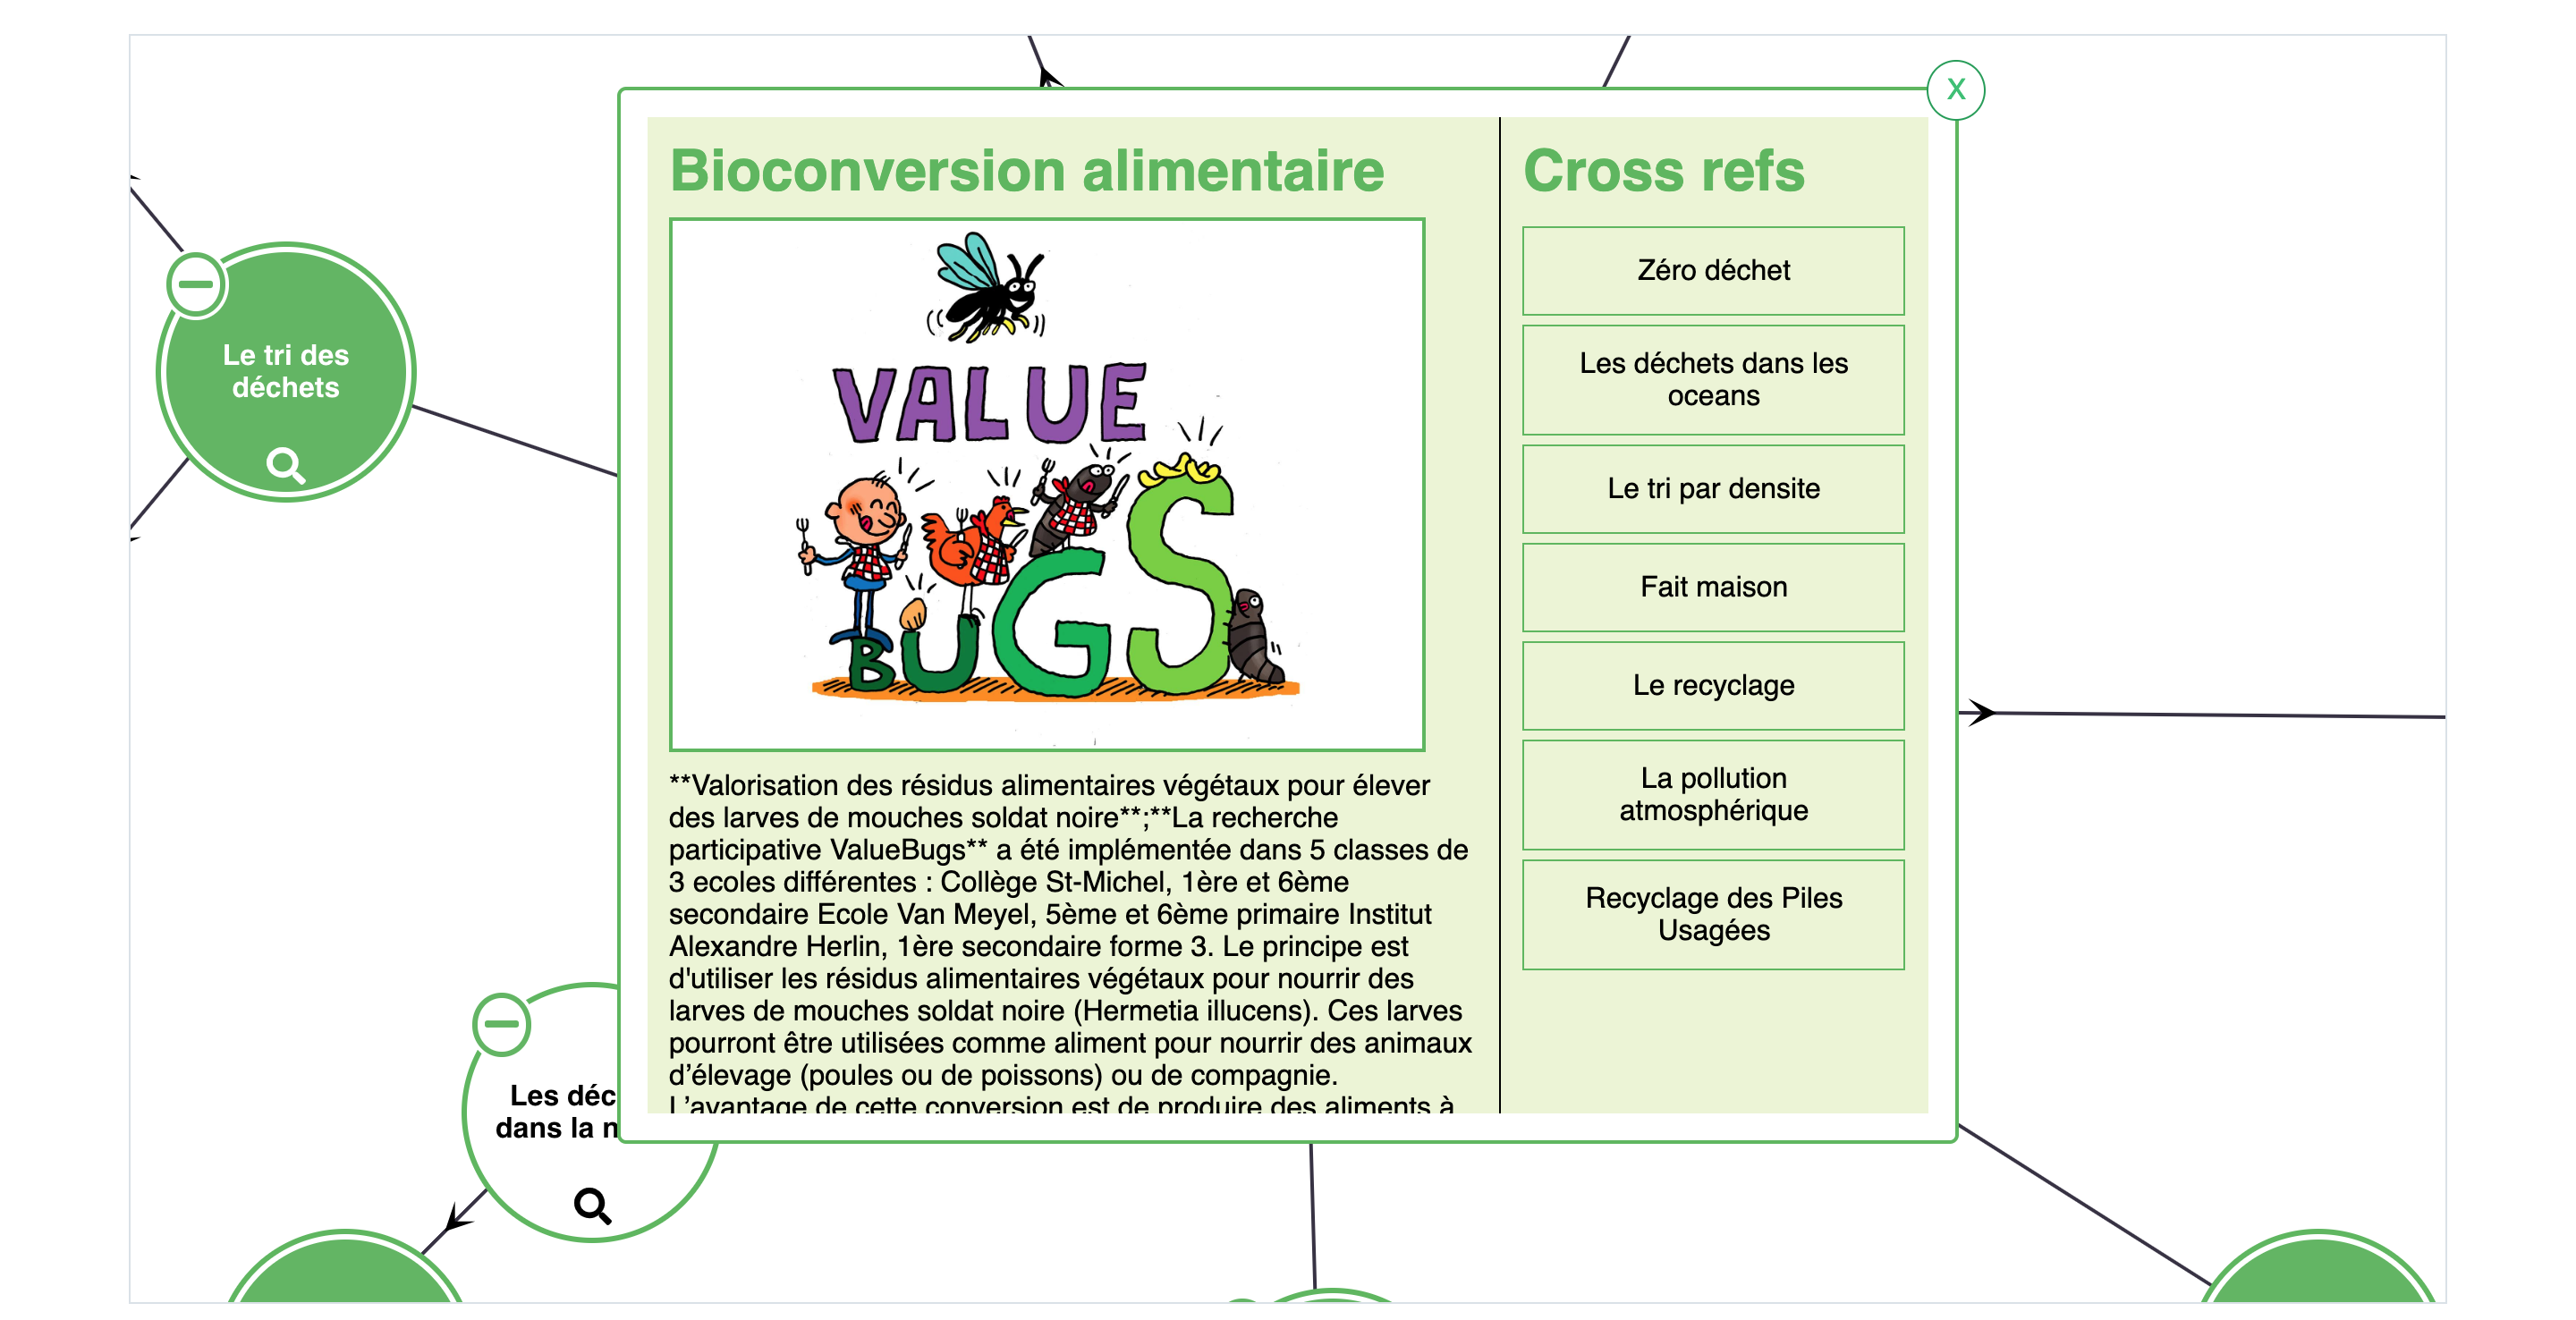
\includegraphics[width=\linewidth]{PDDEditModal.png}}
	\caption{Plateforme DD Edit Modal.}
	\label{fig:pdd-editmodal}
\end{figure}

At the left part of the edit modal, the actual content is shown. It starts with the title of the node, followed by a picture. If no picture exists, the text providing more information about the topic of the node is shown immediately under the title. Otherwise the title and the text are separated by the picture.\\

The size of the edit modal is fixed, but in case the information does not fit the modal, the user can scroll in the left part to continue reading until the end. The modal will not grow in size to make sure all data fits in it.\\

For some nodes, the edit modal will contain a list of so-called ``cross references'', which are links to nodes that in some way are related and which are not a direct child of the node. Such a link is not shown in the visualization, but by providing such a list, the user can still discover them. A click on a cross reference will close the modal and \textit{move} the visualization until the node of the corresponding cross reference is centered. This allows the user to navigate to linked nodes without the need to show a spaghetti of links in the visualization.



\subsection{Action Listeners}\label{sec:usecase-actionlisteners}
In GuideaMaps, we have a controls-div (section \ref{sec:controls}) containing a number of buttons to allow the user to perform some actions. In Plateforme DD, we chose for another approach. Because we have circular nodes instead of rectangular, it is less convenient to position multiple buttons next to each other at the bottom of the node. Further, we don't need a button to add child nodes because this is not allowed in Plateforme DD. Hence, we only have two buttons: one to expand and collapse the child nodes and one to open the edit modal.\\

The button to open the node is positioned in the center at the bottom of the node. A click on that button opens the modal and centers the node such that the node is in the middle of the screen when the user closes the modal. Specific to this implementation is that there is a second way to open the modal. If the user clicks once on the node, it is centered. If he clicks once more on the node (not necessarily on the button), the modal will open and the content will be shown. This is because a click on a centered node results in the same action as a click on the button to open the node.\\

The second button is one to expand or collapse the child nodes. As already said, we cannot position it next to the other button at the bottom of the node. Therefore we position it at the top-left of the boundary of the node. There, a circle is visible with a minus inside if the children are visible. A click on the minus will collapse the node such that the children are not visible anymore and replace the minus by a plus. When the user clicks on that plus again, the exact opposite action will happen: the node will be expanded and hence the children of the node will be visible again and the plus is replaced by a minus.\\

Note that a plus and minus can be used here as symbols to expand and collapse a node. This is possible because there can be no confusion with the action of adding a child node in Plateforme DD. If this would be possible, other symbols should be used to avoid such confusion and to not reduce the intuitiveness (Usability Requirement \ref{item:intuitiveness}).


